\documentclass[12pt]{article}
\usepackage[dvipsnames]{xcolor}
\usepackage{graphicx}
\usepackage{amsmath}
\usepackage{amssymb}
\usepackage[color,matrix,frame,arrow,curve]{xy}
\begin{document}


\begin{figure}[h!]
\centering
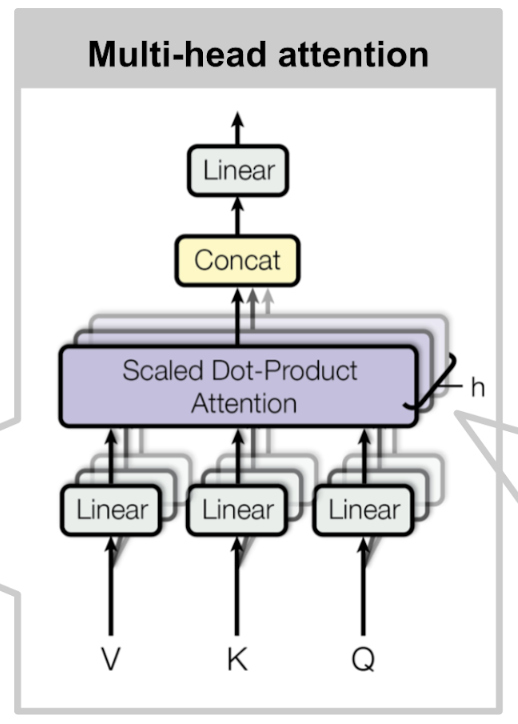
\includegraphics[width=3in]
{multi-head-att.jpg}
\caption{View of Mount Vesuvius from
  Pompeii}
\label{fig-jpg}
\end{figure}


\begin{figure}[h!]\centering
$$\xymatrix{
&&&&*+[F*:SpringGreen]{\underline{L}^{3\times  4}}&&&&
\\
&&&&*+[F*:yellow]{\underline{C}^{3\times  4}}\ar[u]&&&&
\\
&*+[F*:Orchid]{\underline{X}^{3\times  4}}\ar[urrr]&&&*+[F*:Orchid]{\underline{Y}^{3\times  4}}\ar[u]&&&*+[F*:Orchid]{\underline{Z}^{3\times  4}}\ar[ulll]&
\\
*+[F*:SpringGreen]{\underline{1}^{3\times  4}}\ar[ur]\ar[urrrr]\ar[urrrrrrr]&*+[F*:SpringGreen]{\underline{2}^{3\times  4}}\ar[u]\ar[urrr]\ar[urrrrrr]&*+[F*:SpringGreen]{\underline{3}^{3\times  4}}\ar[ul]\ar[urr]\ar[urrrrr]&*+[F*:SpringGreen]{\underline{4}^{3\times  4}}\ar[ull]\ar[ur]\ar[urrrr]&*+[F*:SpringGreen]{\underline{5}^{3\times  4}}\ar[ulll]\ar[u]\ar[urrr]&*+[F*:SpringGreen]{\underline{6}^{3\times  4}}\ar[ullll]\ar[ul]\ar[urr]&*+[F*:SpringGreen]{\underline{7}^{3\times  4}}\ar[ulllll]\ar[ull]\ar[ur]&*+[F*:SpringGreen]{\underline{8}^{3\times  4}}\ar[ullllll]\ar[ulll]\ar[u]&*+[F*:SpringGreen]{\underline{9}^{3\times  4}}\ar[ulllllll]\ar[ullll]\ar[ul]
\\
&*+[F*:Dandelion]{\underline{Q}^{3\times  4}}\ar[ul]\ar[u]\ar[ur]&&&*+[F*:Dandelion]{\underline{K}^{3\times  4}}\ar[ul]\ar[u]\ar[ur]&&&*+[F*:Dandelion]{\underline{V}^{3\times  4}}\ar[ul]\ar[u]\ar[ur]&
}$$
\caption{Multi-head Attention}
\label{fig-texnn-for-multi-head-att}
\end{figure}\begin{subequations}
\begin{equation}
Q^{3\times  4} =)
\label{eq-Q-fun-multi-head-att}
\end{equation}

\begin{equation}
K^{3\times  4} =)
\label{eq-K-fun-multi-head-att}
\end{equation}

\begin{equation}
V^{3\times  4} =)
\label{eq-V-fun-multi-head-att}
\end{equation}

\begin{equation}
1^{3\times  4} = {\rm linear}(Q^{3\times  4})
\label{eq-1-fun-multi-head-att}
\end{equation}

\begin{equation}
2^{3\times  4} = {\rm linear}(Q^{3\times  4})
\label{eq-2-fun-multi-head-att}
\end{equation}

\begin{equation}
3^{3\times  4} = {\rm linear}(Q^{3\times  4})
\label{eq-3-fun-multi-head-att}
\end{equation}

\begin{equation}
4^{3\times  4} = {\rm linear}(K^{3\times  4})
\label{eq-4-fun-multi-head-att}
\end{equation}

\begin{equation}
5^{3\times  4} = {\rm linear}(K^{3\times  4})
\label{eq-5-fun-multi-head-att}
\end{equation}

\begin{equation}
6^{3\times  4} = {\rm linear}(K^{3\times  4})
\label{eq-6-fun-multi-head-att}
\end{equation}

\begin{equation}
7^{3\times  4} = {\rm linear}(V^{3\times  4})
\label{eq-7-fun-multi-head-att}
\end{equation}

\begin{equation}
8^{3\times  4} = {\rm linear}(V^{3\times  4})
\label{eq-8-fun-multi-head-att}
\end{equation}

\begin{equation}
9^{3\times  4} = {\rm linear}(V^{3\times  4})
\label{eq-9-fun-multi-head-att}
\end{equation}

\begin{equation}
X^{3\times  4} = {\rm scaled\_dot\_prod\_att}(1^{3\times  4},2^{3\times  4},3^{3\times  4},4^{3\times  4},5^{3\times  4},6^{3\times  4},7^{3\times  4},8^{3\times  4},9^{3\times  4})
\label{eq-X-fun-multi-head-att}
\end{equation}

\begin{equation}
Y^{3\times  4} = {\rm scaled\_dot\_prod\_att}(1^{3\times  4},2^{3\times  4},3^{3\times  4},4^{3\times  4},5^{3\times  4},6^{3\times  4},7^{3\times  4},8^{3\times  4},9^{3\times  4})
\label{eq-Y-fun-multi-head-att}
\end{equation}

\begin{equation}
Z^{3\times  4} = {\rm scaled\_dot\_prod\_att}(1^{3\times  4},2^{3\times  4},3^{3\times  4},4^{3\times  4},5^{3\times  4},6^{3\times  4},7^{3\times  4},8^{3\times  4},9^{3\times  4})
\label{eq-Z-fun-multi-head-att}
\end{equation}

\begin{equation}
C^{3\times  4} = {\rm concat}(X^{3\times  4},Y^{3\times  4},Z^{3\times  4})
\label{eq-C-fun-multi-head-att}
\end{equation}

\begin{equation}
L^{3\times  4} = {\rm concat}(C^{3\times  4})
\label{eq-L-fun-multi-head-att}
\end{equation}

\end{subequations}


\end{document}  
